\documentclass{article}
\usepackage[utf8]{inputenc}
\usepackage[right=2cm,left=3cm,top=2cm,headsep=0.5cm,footskip=0.5cm]{geometry}

\title{The Impossible  Early Galaxy Problem}
\author{Santiago Arranz Sanz }
\date{June 2019}

\usepackage{natbib}
\usepackage{graphicx}
\usepackage{latexsym}
\usepackage{eufrak}
\usepackage{dsfont}
\usepackage{hyperref}
\usepackage{enumerate} 
\usepackage{lscape}
\usepackage{titlesec}
\usepackage{fancyhdr}
\usepackage{color}
\usepackage{cleveref}

\crefformat{section}{\S#2#1#3} % see manual of cleveref, section 8.2.1
\crefformat{subsection}{\S#2#1#3}
\crefformat{subsubsection}{\S#2#1#3}


\newtheorem{teo}{\underline{Teorema}}
\newtheorem{defi}{\underline{Definici\'on}}
\newtheorem{propo}{\underline{Proposici\'on}}
\newtheorem{ejem}{\underline{Ejemplo}}[section]
\newtheorem{prob}{\underline{Problema}}
\newtheorem{lema}{\underline{Lema}}
\newtheorem{obs}{\underline{Observaci\'on}}
\newtheorem{ide}{\underline{Idea}}

\begin{document}

\maketitle

\section*{Introduccion}

Después de leer varios artículos en los que trata dicho problema y derivados he llegado a la conclusión que el problema base es la discordancia del modelo actual de fusión jerárquica con la falta de observación de galaxias transitorias entre los halos iniciales y las galaxias más masivas en los redshift $z\sim 4-6$. Veamos algunos resumenes de los artículos principales.

\section{The Impossible Early Galaxy Problem}
\citep{steinhardt2016impossibly} Según el paradigma actual de la fusión jerárquica de galaxias en el modelo cosmológico estandar, en torno a los redshift $z\sim 4-6$ ha de existir la transición de las galaxias más masivas desde los halos iniciales que acretan masa a las últimas fases de evolución bariónica vista en las galaxias con formación estelar y \textit{quasars}. Sin embargo, ninguna evidencia ha sido encontrada en muchos estudios a alto redshift como el CFHTLS, CANDELS y el SPLASH, los primeros estudios para probar la masa alta final en estos redshift. Considerando que el ratio masa estelar- masa halo (SMHMR) estimado a bajo redshift permaneciera constante en $z\sim 6-8$, CANDELS y SPLASH darían mayores ordenes de magnitud de número de halos de masa $M\sim 10^{12-13}M_\odot$ que los que se podrían haber formado a esos redshift, esto se conoce como el problema de la galaxia masiva temprana imposible. En el artículo de \cite{steinhardt2016impossibly} consideran los posibles errores sistemáticos que puedan explicar esta contradicción de teoría y observaciones en los modelos de síntesis estelar usados para estimar los parámetros físicos  y en los escenarios posibles de formación galáctica. Es posible que las incertidumbres desconocidas reduzcan la disparidad entre observaciones y simulaciones de CMD tomando una visión conservadora de las observaciones,aun así existirían tensiones considerables con la teoría.\\

Existe un consenso bastante amplio en la distribución de masa y redshift de los halos producidos en el colapso inicial de las pequeñas fluctuaciones de densidad en el universo temprano y el modelo de fusión jerárquico. Para la cosmología estándar la función de masa es sencilla de calcular. Este consenso se basa en la idea de la rápida evolución en la densidad de halos masivos en $z>4$ que deberían ser observacionalmente evidente en las funciones de masa y luminosidad galácticas. Hasta hace poco el catálogo de galaxias a redshift $z>6$ era limitado y sesgado a las galaxias más brillantes, galaxias individuales masivas y \textit{quasars}. Sin embargo con los nuevos estudios como el CANDELS o el SPLASH se ha podido probar la función de luminosidad y de masa para galaxias en el rango de $z\sim 4-8$, lo que nos permite calcular la función de masa del halo correspondiente a dicho rango.\\

Trabajos como el de \cite{finkelstein2015increasing} muestra las tensiones ocasionadas en $z>4$ entre la evolución esperada de la función de masa del halo y las funciones de luminosidad y de masa de las galaxias.\footnote{El resumen de dicho trabajo lo podemos encontrar en \cite{arranz2015finkelstein}} \\

\section{Galaxias tempranas y sus halos}
Como hemos visto en el trabajo de \cite{finkelstein2015increasing} la teoría espera una rápida evolución en las galaxias entre los redshift de $z=4-7$, sin embargo las observaciones no avalarón dichas prediccionas en su trabajo. En el trabajo de \cite{steinhardt2016impossibly} pretende extender y actualizar los resultados de trabajos como el de \cite{finkelstein2015increasing} basándose en los datos de CANDELS y SPLASH. La ventaja de tomar redshift altos como los del estudio de $z=4-8$ es que tenemos un tiempo cósmico más pequeños (0.9 Gyr \citep{steinhardt2016impossibly}) en un mayor número de redshift, lo que debiese permitir ver una evolución mas detallada que en redshift bajos. Por otro lado los métodos de estimación de las masas de los halos son menos abundantes por lo que el trabajo de \cite{steinhardt2016impossibly} trabaja básicamente con tres tipos de estimaciones.
\begin{enumerate}
\item El primero de ellos se base en la clusterización \citep{hildebrandt2009cars} el cual estima la masa del halo según la distribución espacial de las galaxias. La ventaja de este método es que no hay que asumir ninguna propiedad física de las galaxias, pero sí es necesario escoger un modelo de materia oscura para las simulaciones.
\item Un segundo método es el presentado y desarrollado en el artículo de \cite{finkelstein2015increasing}, el cual se basa en la curva de luminosidad UV \footnote{Hay que recordar que podría ser incorrecta ya que en el artículo de se asumio la existencia de galaxias solo visibles en submilimétricas \citep{wang2019dominant}.} y en la función de masa calculada a través de simulaciones, relacionando ambas por el principio de que el halo más masivo a de albergar la galaxia más masiva y viceversa.
\item El último método es asumir un ratio entre luminosidad/masa estelar y materia oscura. El ratio asumido es el redshift más bajos donde las estimaciones de materia oscura son más factibles por los métodos de agrupación. El ratio usado para el enlace entre masa estelar y de halo es  $M_h/M_\star \sim 70 $.
\end{enumerate}

\textcolor{red}{Sobre el primer método no puedo decir mucho de momento ya que no he leido el paper de \cite{hildebrandt2009cars} donde desarrollan el método, pero al igual que en el último método depende de un modelo de materia oscura lo cual podría ser una variable a tener en cuenta para que los resultados cuadren con las observaciones. Sobre el segundo método ya se ha discutido los posibles fallos en \cite{arranz2015finkelstein} que puede tener sobre todo a raiz del descubrimiento de \cite{wang2019dominant}. Por último considera un ratio igual a redshift más bajos lo cual no tendría porque ser cierto si las propiedades de galaxias y halos evolucionan con el tiempo, lo que podría demostrar el artículo de \cite{wang2019dominant} contradiciendo las suposiciones realizadas en \cite{finkelstein2015increasing}. Todos estos puntos débiles pueden ser clave fundamental para poner en duda dichos resultados.}\\

\begin{figure}[h]
\begin{center}
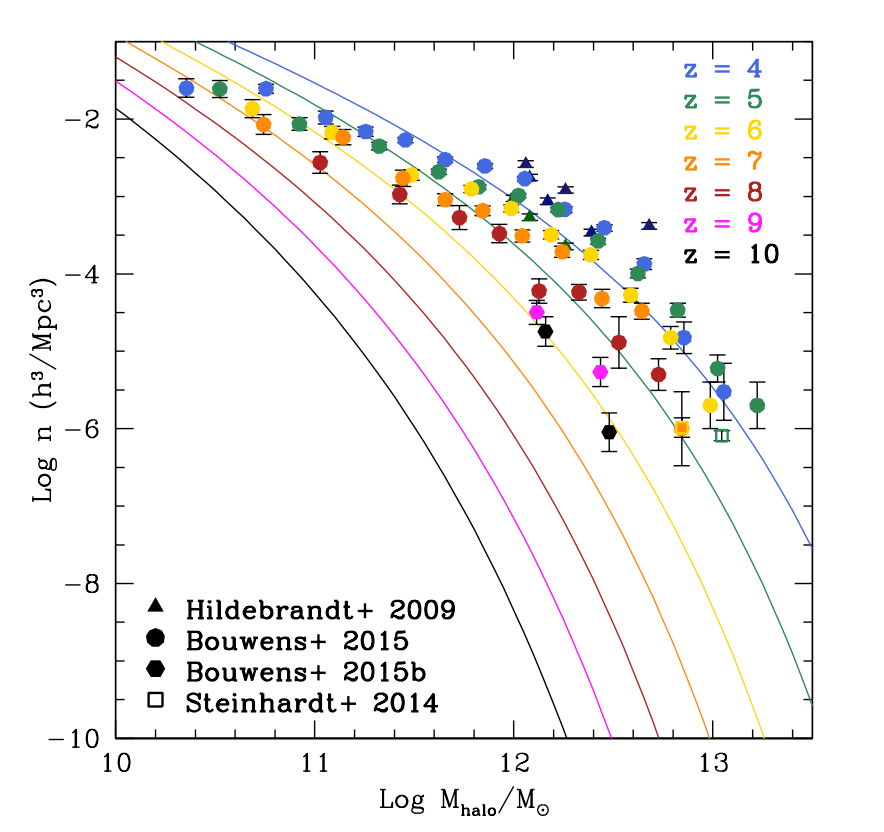
\includegraphics[scale=0.55]{Figuras/steindhart_fig1.png}
\caption{\label{fig:steindhart_fig1} Imagen que representa las estimaciones teoricas del número de densidad de halos en función de su masa versus las obtenidas de las observaciones estudiadas en \cite{steinhardt2016impossibly}}
\end{center}
\end{figure}

Las estimaciones teóricas de la función de masa de los halos para los diferentes redshift han sido sacadas de la herramienta \cite{murray2013hmfcalc} la cual esta basada en el trabajo \cite{sheth2001ellipsoidal}. Las discrepancias que se pueden observar en la \textbf{Figura \ref{fig:steindhart_fig1}} son muy visibles, en especial se encuentran la función de masa del halo de las observaciones tienen un mayor número de densidad de halos masivos con respecto a los predichos por la teoría. Una posible explicación es que el ratio $M_h/L_{UV}$ en galaxias masivas decrece bruscamente en $z>4$, tendiendo a sobrestimar la masa de halos de las galaxias de alto redshift. Si esto fuera así se podría esperar que esta rápida evolución tuviera que ser evidente en otras propiedades medibles de la población de galaxias. En el siguiente punto del artículo de \cite{steinhardt2016impossibly} trata esta posibilidad sin encontrar ninguna evidencia de dicha evolución del ratio de masa halo y luminosidad. \textcolor{red}{Esta posibilidad solo explicaría las medidas basadas en luminosidad, quedando fuera quizás el primer método de clusterización. Por otro lado, la evolución drástica en luminosidad podría hacer que no se viesen todas las galaxias del halo \citep{wang2019dominant} por lo que afectaría a las medidas basadas en clusterización del primer método}

\section{Aspecto normal de las galaxias en alto redshift}
Se ha denominado como \textit{Impossible early galaxy problem} a la brusca discrepancia de las estimaciones de la función de masa de halo entre las observaciones y teorias. Esta discrepancia podría explicarse si no asumimos que el comportamiento de las galaxias en redshift altos es similar a las de bajo redshift, esto podría dar una solución sencilla al problema. Si encontráramos diferencias entre las galaxias de alto y bajo redshift, que permitieran suponer que no es correcto adoptar plantillas de ajustes del SED y relaciones de escala tomadas en redshift bajos en galaxias de altos redshift, podríamos poner en cuestión las estimaciones observacionales que relajarían la tensión con la teoría. \textcolor{red}{Este creo que es el principal punto, veamos como encaja las nuevas observaciones de \cite{wang2019dominant} en este marco y si son relevantes en este punto}\\

En las últimas décadas se ha observado que muchos procesos, incluyendo la formación estelar, ocurre mas temprano en las galaxias más masiva que en las menos masivas. La evolución temprana de las galaxias masivas y con formación estelar es también soportada por la observación de galaxias masivas y pasivas en redshift $z\sim 2-4$. Además, los ratios de FeII/MgII en quasars de alto redhistf y las edades derivadas de los ajustes de los SED sugieren que las galaxias masivas y tempranas necesitan formas sus estrellas más rápidamente.\\

Por otro lado, la teoría $\Lambda$CDM necesita que los halos más masivos generalmente acreten más tarde la matería que sus compañeros menos masivos. Por tanto, reconciliar la teoría y las observaciones requiere que las galaxias más masivas puedan evolucionar más rápido que las menos masivas. Ya que el tiempo dinámico incrementa con la masa, una evolución rápida en redshift altos podría necesitar de que la física de los procesos bariónicos que dominan la formación estelar sea modificada con respecto a redshift más bajos. Por tanto en el modelo se debería predecir que en el intervalo de redshift $z\sim 4-8$ una rápida transición entre los procesos de acreción de los halos y el rápido crecimiento de las poblaciones estelares. \\

\textcolor{red}{Observamos otra discrepancia entre teoría y observación, si la acreción de masa en los halos masivos tiene un mayor tiempo de duración que en los más pequeños en estos últimos el gas se debería de enfriar antes y deberían de poder formar estrellas con más rapidez. Sin embargo, se observa que las galaxias más masivas (asociadas a los halos más masivos) forman sus estrellas más rápido que los menos masivos (asociados a los menos masivos). Al igual que ocurre en el análisis de \cite{finkelstein2015increasing} \citep{arranz2015finkelstein} entra en cuestión la suposición de que las galaxias más masivas se encuentran en los halos más masivos, quizás las dinámicas en la acrección de masa en los halos masivos impidan la formación de galaxiás masivas, produciendo una mayor cantidad de galaxias menos masivas quedando las galaxias masivas en halos menos masivos. Esto debería de indicar una relación masa halo y masa estelar menor de lo esperado lo cual podría ser estudiado con RAMSES. Por otro lado, tomando por buena esta suposición se deduce que los procesos de la física barionica implicados en la formación estelar han de ser distintos en redshift altos, por ejemplo los tiempos de enfriamiento, lo cual debería de dejar una señal entre las galaxias de redshift 4 y 8.}\\

\subsection{Similitudes de la relación SFR-Masa estelar entre galaxias de alto y bajo redshift.}

Hasta la fecha, CANDELS y SPLASH no han encontrado desviaciones aparentes de las propiedades derivadas en redshift bajos. En cambio, encuentran que la tendencia a que más y más galaxias masivas evolucionen antes continúa hasta $z \sim 6 - 8$. En particular, a $0< z <4$ se ha demostrado que las galaxias formadoras de estrellas se encuentran en una "secuencia principal" \citep{Renzini_2015}, con una estrecha correlación entre la masa estelar existente y su tasa de formación de estrellas. Un análisis de más de dos docenas de estudios de galaxias formadoras de estrellas utilizando diferentes técnicas para la selección, para medir la masa estelar y para medir la tasa de formación de estrellas muestra un fuerte acuerdo en la evolución de la pendiente y el desplazamiento al rojo.
Las primeras galaxias de alto desplazamiento al rojo se encuentran en la extrapolación de esta secuencia principal a $z \sim 6-7$.\\

La secuencia principal de formación estelar está bien medida para objetos de menor masa en $z\sim 5-6$ entre SPLASH y CANDELS. Donde hay masas estelares disponibles, las galaxias tempranas más masivas se encuentran directamente en la extrapolación de gran masa de esta secuencia principal. Debido a que la masa estelar y las tasas de formación de estrellas se miden usando diferentes longitudes de onda, los errores sistemáticos del ajuste incorrecto de la plantilla producirían cantidades inferidas incorrectas de diferentes maneras, y probablemente producirían una población inconsistente con la secuencia principal. Del mismo modo, los problemas de desmembramiento arbitrario producirían valores atípicos ubicados en algún lugar arbitrario y, por lo tanto, probablemente fuera de esta secuencia principal. \textcolor{red}{Diferentes medidas en diferentes longitudes de ondas nos llevan al mismo resultado, en el caso de haber errores sistemáticos cada una de esas medidas tendrían un error y por tanto los resultados serían muy aleatorios. Entiendo que es ese el argumento dado.} \\

La evolución de desplazamiento al rojo de la secuencia principal de formación estelar también se entiende bien en $0<z<4$, y la secuencia principal de formación de estrellas $4<z<6$ observada tiene las propiedades producidas extrapolando esa dependencia del tiempo. El aumento de la masa hacia el alto desplazamiento al rojo de las N galaxias formadoras de estrellas más masivas (un componente de lo que se ha denominado el problema de ``\textit{downsizing}''\footnote{El problema de \textit{downsizing} trata que los moedelos actuales de fomración galáctica predicen que las primeras galaxias formadas son las de baja masa mientras que en las observaciones se ven que las galaxías con poblaciones mas antiguas de estrellas son las más masivas. Se ve ademas en redshift altos que las formadoras de estrellas son las galaxias masivas cuando en teoría deberían de ser las menos masivas.}) también está bien medido, y las galaxias formadoras de estrellas más masivas en $z\sim6$ se encuentran en la extrapolación de la dependencia del tiempo de mejor ajuste en $0<z<4$ (\textbf{Figura \ref{fig:steindhart_fig2}}). \textcolor{red}{La \textbf{Figura \ref{fig:steindhart_fig2}} Parecer mostrar muy claramente dicha relación, se ve una relación lineal muy estrecha aunque pudiera ser por selección de datos.} \\

\begin{figure}[t]
\begin{center}
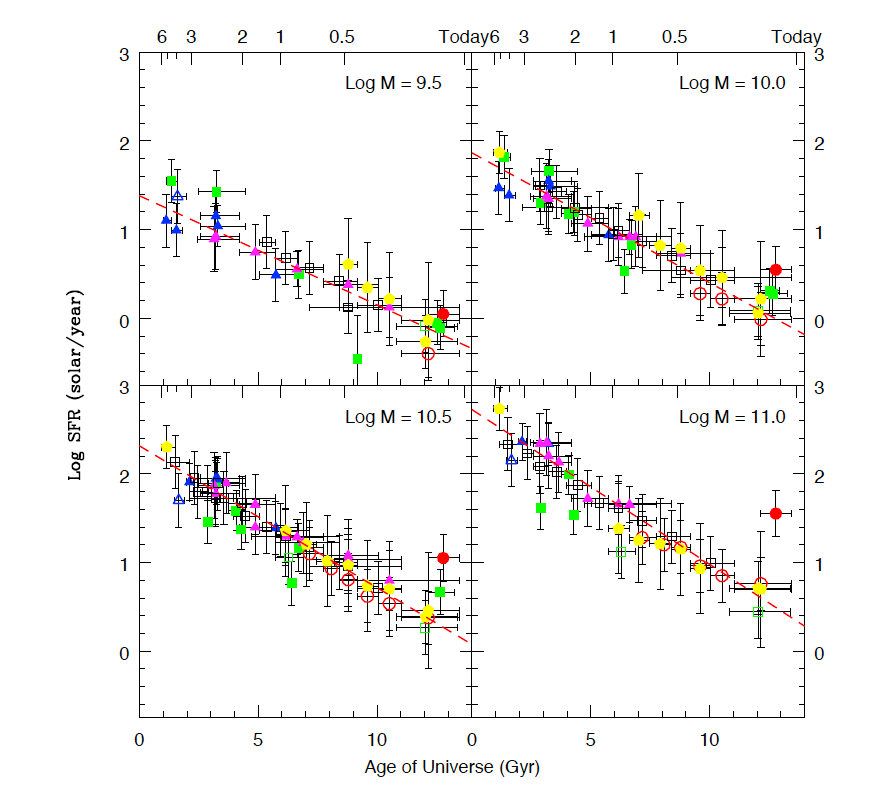
\includegraphics[scale=0.65]{Figuras/steindhart_fig2}
\caption{\label{fig:steindhart_fig2} 96 mediciones de 32 estudios de la secuencia principal de formación de estrellas 4 para $M_\star$ fijo $= 10^{10.5}M_\odot$ a $0 <z <6$, ajustado para ubicarse en un conjunto común de calibraciones siguiendo la prescripción derivada por \cite{speagle2014highly} utilizando 25 de estos estudios. Las barras horizontales indican el rango de redshift que abarca cada observación en particular, mientras que los errores verticales son la verdadera dispersión sobre cada observación de la secuencia principal \citep{speagle2014highly}. Aunque estos estudios utilizan muchos métodos diferentes para determinar la SFR y la masa estelar (azul = UV, púrpura = UV + IR, rojo = IR, verde = líneas de emisión, amarillo = ajuste SED, negro = radio), todos muestran un buen acuerdo con  la evolución lineal de mejor ajuste (log) determinada en $0 <z <4$ (línea de puntos), y las mediciones del redshift más altas son consistentes con la extrapolación de ese ajuste a $z\sim 6$. Por lo tanto, parece probable que las técnicas para estimar estelares las masas y las tasas de formación estelar no se han vuelto catastróficamente incorrectas en $z\sim 6$.}
\end{center}
\end{figure}

En algún momento, las plantillas estelares derivadas de un desplazamiento hacia el rojo bajo dejarán de ser válidas, pero esto aún no se ha observado. Podría esperarse que esto ocurra solo cuando la física de la formación estelar haya cambiado, tal vez debido a unas metalicidades muy bajas que producen un IMF muy pesado e incluso estrellas de la Población III \footnote{¿Sobre redshift $z\sim 20$?}. Si es así, las plantillas pueden seguir siendo válidas muy por encima de $z\sim 6-8$. Como mínimo, parece claro que no se han vuelto catastróficamente incorrectos en el rango de desplazamiento al rojo donde se han medido imposiblemente las primeras galaxias.\\

\textcolor{red}{El \textit{downsizing} parece otra cara del mismo problema. En \citep{arranz2015finkelstein} se vió el problema de que la densidad de galaxias masivas luminosas parecía mantenerse en el rango de redshift $4<z<7$ mientras que el número de densidad de galaxias bajaba con el aumento del redshift. Parecía que las galaxias luminosas se mantienen siendo estás las primeras en formar estrellas, al contrario de lo que predice la teoría y las simulaciones. La pregunta es si falla la teoría, las observaciones o ambas opciones.}

\subsection{Relación Galaxia - Quasar}

Al igual que ocurre con el número de galaxias de formación estelar, la presencia de quasares plantea un problema similar en redshift altos, ya que parecen ser más lusminosos y con agujers negros más masivos con un mayor redshift. Este problema se ha conocido como ``\textit{impossibly early black hole}'' de manera análoga al problema que estamos estudiando.\\

Una parametrización de la similitud entre la evolución del redshift de los cuásares y las galaxias formadoras de estrellas es observar que la relación de $M_\star$ para la mayoría de las galaxias formadoras de estrellas masivas con respecto a $M_{BH}$ para los cuásares más masivos se observa que es aproximadamente $30:1$ en todo redshift fijo. Las galaxias $log M_\star / M_\odot\sim11.2$ en $z\sim 6$ en SPLASH tienen una relación similar con los primeros cuásares masivos, como el quasar $log M_{BH} / M_\odot\sim 10.08$  en $z = 6.4$ estudiado en \cite{wu2015ultraluminous}. Porque las estimaciones de masa del agujero negro virial tienen incertidumbres sistemáticas muy diferentes a las estimaciones de masa estelar, esta relación que sigue siendo una evidencia adicional de que las propiedades inferidas para las galaxias imposiblemente tempranas son probablemente razonables.\\

Se espera que a un redshift lo sufucientemente grande varias de estas relaciones de escala se vengan a bajo, pero aún no se ha podido observar. El punto clave es que la población observada de galaxias formadoras de estrellas  en redshift altos  sigue la evolución esperada hacia el redshift determinada observacionalmente a partir de muchos estudios de redshift más bajo. Incluso los objetos más masivos y de redhift más altos se encuentran y analizan utilizando las mismas técnicas estándar que se ha verificado que tienen éxito en el redshift más bajo,siendo extraños únicamente por la discrepancia entre la observación y el $\Lambda$CMD, no por los datos.\\

\textcolor{red}{Parece haber una reticencia en el artículo en admitir la posibilidad de que las técnicas de análisis que se aplican en redshift bajos no sean válidas en redshift altos. No me queda del todo claro como se mide la similitud de las propiedades de galaxias en bajo y alto redshift, tampoco como se realiza la extrapolación de las características de bajo redshift a alto redshift que tanto se citan. Por otro lado la \textbf{Figura \ref{fig:steindhart_fig2}} parece mostrar perfectamente la relación mostrada en la secuencia principal, donde el slope parece mantenerse (creciendo con el redshift) y aumentar el punto de intersección con una mayor masa estelar.}

\section{Función de luminosidad para determinar la masa del Halo.}
Las funciones de luminosidad UV son una de las más baratas y más robustas observaciones para obtener en redshift altos y se pueden convertir en masas de halo suponiendo una relación de masa a luz de halo. De hecho, la mayoría de los datos de alto redshift que se muestran en la \textbf{Figura \ref{fig:steindhart_fig1}} y todos aquellos en $z> 6$ se derivan de las funciones de luminosidad UV monocromática , las únicas observaciones disponibles. La principal ventaja de esta técnica sobre las funciones de masa es que coloca la mayor parte de la incertidumbre potencialmente grande en la relación masa-luz del halo, que se puede parametrizar en un solo modelo donde se puede analizar con mayor claridad. En contraste, las funciones de masa colocan gran parte de la incertidumbre en los detalles del conjunto diverso de modelos de distribución de energía espectral que se ajustan a cada galaxia individual donde pueden ser difíciles de entender.\\

Además de la incertidumbre en la correspondencia entre la masa del halo y la luminosidad UV, la comparación de la observación con la teoría también requiere observaciones coincidentes de las galaxias en medio de la formación de estrellas con predicciones teóricas sobre el momento en que se formó su halo. Después de todo, las galaxias probablemente no emergen completamente formadas en el momento en que un halo se virializa; la materia oscura simplemente tiene que colapsar gravitacionalmente, mientras que los bariones comienzan más tarde en pequeñas masas y deben agruparse y enfriarse para formar estrellas. Si este proceso generalmente toma, por ejemplo, 300 Myr para cada galaxia debido a consideraciones dinámicas, entonces un aumento brusco en la función de masa de halo como se predice del redshift 8.0 a 4.0 conduciría a un aumento brusco en la función de luminosidad UV para las galaxias correspondientes del redshift 6.0 a 3.4. Más generalmente, en un universo dominado por la materia, $dz / dt \propto t^{-5/2}$. Por lo tanto, los retrasos entre el halo ($t$ más pequeño) y la formación de galaxias ($t$ más grande) conducen a que la función de luminosidad UV evolucione igualmente rápida con el tiempo pero en un rango más pequeño en el redshift, produciendo un efecto más notable observacionalmente (\textbf{Figura \ref{fig:steindhart_fig3}}). \\

\begin{figure}[t]
\begin{center}
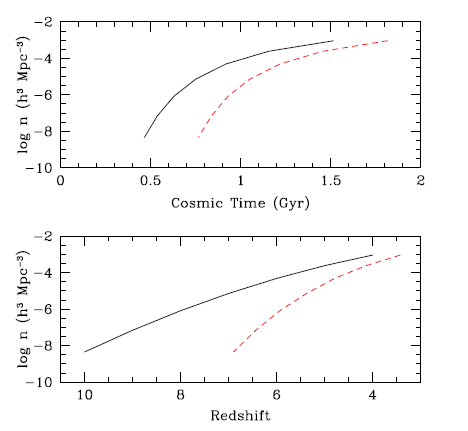
\includegraphics[scale=0.65]{Figuras/steindhart_fig3}
\caption{\label{fig:steindhart_fig3}  Densidad numérica de $10^{12}M_\odot$ halos (negro, sólido) a partir de predicciones teóricas y densidad numérica correspondiente (es decir, punto en una función de luminosidad) ) para galaxias formadoras de estrellas (rojo, punteado) para un modelo de prueba en el que las estrellas forman 300 Myr después de la virialización del halo. Hay un momento característico para formar tales halos, visto como un fuerte aumento en la densidad numérica a lo largo del tiempo (arriba) o hacia un redshift más alto (abajo). Aunque el aumento en la densidad numérica de halos y (300 Myr más tarde) de galaxias es igualmente rápido en el tiempo, debido a la relación edad-redshift, el aumento en las galaxias, que tiene lugar en un momento posterior y un redshift más bajo , parece más agudo con respecto al desplazamiento hacia el rojo. Debido a que la evolución de las funciones de masa y luminosidad se muestra típicamente en términos de evolución hacia el redshift, esto significa que un fuerte aumento en la densidad numérica de halos parece producir una evolución aún más aguda observada en la función de luminosidad correspondiente.}
\end{center}
\end{figure}

El retraso de tiempo entre el acreción de la masa del halo y la evolución estelar posterior depende de la relación entre la formación de halo y la evolución de las galaxias que evolucionan dentro de esos halos. Restringir la relación de luminosidad a masa de halo implica restringir la función de masa inicial de alto redshift, el contenido de polvo y otros procesos involucrados en la formación de las primeras grandes poblaciones estelares formadas por galaxias.\\

Debido a que hay muy poca degeneración entre los cambios de masa y tiempo, si tanto la función de luminosidad UV como la función de masa de halo se miden bien de forma independiente, debería ser posible determinar ambos cambios. De hecho, tal determinación es la idea central detrás del emparejamiento de abundancia, usando una combinación de predicciones teóricas y medidas de densidad numérica para ``emparejar'' halos con galaxias (por ejemplo, \cite{finkelstein2015increasing}). Sin embargo, lo que encontramos es que este proceso de emparejamiento parece fallar en el redshift alto. Como se muestra en la \textbf{Figura \ref{fig:steindhart_fig1}}, hacer coincidir los halos con las galaxias requeriría que las galaxias vivan en halos tan pequeños que no sean físicamente posibles, en casos extremos menos de un factor de tres más alto que las masas estelares. -la evolución masiva en la función de masa de halo no ha tenido contrapartida observada en las funciones de luminosidad, ya sea en redshift alto o durante un período de tiempo similar en redshift más bajo.

\subsection{Ratio masa Halo - función de luminosidad.} \label{sec:ratio_halo_lum}
Fuera de $z = 4.7$, varios estudios son consistentes con una relación de masa a luz casi constante de halo. Sin embargo, esta relación debe evolucionar a redshift más altos para conciliar la función de luminosidad UV con la fusión jerárquica (\textbf{Figura \ref{fig:steindhart_fig1}}). Esto puede ocurrir de dos maneras: los halos podrían ser más eficientes en producir estrellas de lo que se creía anteriormente o las estrellas podrían producir más luz UV por unidad de masa estelar que a un redshift más bajo.\\

Para determinar la mejor explicación, consideremos el tamaño del cambio en la relación de masa de halo a luminosidad que se requeriría para conciliar la observación con la teoría. A una luminosidad monocromática fija de, por ejemplo, $M_{1600, AB} = -21$, hay una disminución de 1.5 dex en la densidad numérica de $z = 4$ a 8. En $z\sim 4$, el análisis de agrupamiento muestra que esto corresponde a una masa de halo de $\log M_{Halo} / M_\odot = 12.4$ en un escenario optimista, en el que las estrellas nacen instantáneamente para que no haya retraso de tiempo entre la formación de halo y galaxia, la densidad numérica observada para $M_{1600, AB} = -21$ galaxias en $z = 8$ corresponde a la densidad numérica de $\log M_{Halo} / M_\odot = 11.6$ halos. Por lo tanto, se requeriría una fuerte evolución de 0.8 dex en $M_{Halo} / L_{UV}$ de $z = 4$ a 8. Consideramos en el resto de esta sección si esta evolución es plausible.

\subsection{Modelos de evolución estelar}
La evolución en la relación de masa a luz del halo se consideraría dominada por cuatro efectos:
\begin{description}
\item[Evolución Estelar:] En una población estelar típica, la luminosidad está dominada por estrellas masivas, pero la masa estelar (que se usa para estimar la masa de halo) está dominada por estrellas de baja masa. Como resultado, la relación de masa a luz es mayor para las poblaciones estelares más antiguas. Suponiendo que las galaxias en z = 8 tienen poblaciones estelares más jóvenes que z = 4, este efecto actúa en la dirección de conciliar la observación con la teoría. El aumento de la metalicidad asociada con la maduración de las poblaciones estelares aumenta este efecto.

\item[Cambios de IMF:] Si la función de masa inicial (IMF) es muy pesada en el redshift alto, como se esperaba para las estrellas Pop.III, esto nuevamente actuaría para disminuir la relación de masa a luz. Sin embargo, se espera que el IMF sea similar en todos los $z <8$ basado en sistemas aparentemente análogos de bajo redshift (Dias et al. 2010), y por lo tanto no tendrá impacto en galaxias imposiblemente tempranas.

\item[Evolución de las correciones del polvo:] Muy pocas galaxias con fotometría $z> 4$ se seleccionan como altamente polvorientas, por lo que no es plausible una fuerte reducción en la extinción de los modelos actuales. Sin embargo, si estuvieran polvorientos, un aumento en la extinción aumentaría la relación entre la masa del halo y la luminosidad monocromática UV, haciendo que los halos que contienen galaxias tempranas sean aún más masivos de lo que se mide actualmente. \textcolor{red}{Esre podría ser el caso de las galaxias descubiertas por \cite{wang2019dominant}}.

\item[Fusiones y tiempos:] La agrupación y la fusión dan como resultado la acrección de masa de halo y masa estelar a las galaxias, así como gas adicional que eventualmente formará estrellas. Una fusión de dos objetos grandes con la misma relación masa-luz producirá una galaxia con esa misma relación. Sin embargo, una acumulación más gradual tanto de la materia oscura como del gas capaz de formar estrellas producirá un aumento inmediato de la masa de halo pero un aumento retardado de la masa estelar, lo que hará que la típica relación masa-luz del halo sea mayor en z = 8 que en z = 4 Esto actuaría en la dirección de empeorar el problema, porque las galaxias con la misma luminosidad ahora residirían en halos aún más masivos, que tienen una densidad numérica más baja y un tiempo de virialización posterior. Por ejemplo, \cite{behroozi2015simple} encuentran que una galaxia de $10^{10}M_\odot$ en $z = 7$ debería corresponder a un halo de $10^{12.9}M_\odot$, mientras que asumimos, según las mediciones de redshift más bajo, que su halo estaba por debajo de $10^{12}M_\odot$.
\end{description}

Escogiendo las situaciones más favorables para nuestro objetivo de cuadrar las observaciones con la teoría no se ha podido llegar a resultados satisfactorios. En todos los modelos probados las observaciones dan valores por encima de lo que predice la teorías.

\subsection{Otras posibilidades}
¿Hay otras formas de cambiar rápidamente la relación de masa de halo a luminosidad UV para explicar el desajuste observado? Una posibilidad es permitir una rápida evolución en la función de masa inicial (IMF). Se espera que la IMF sea sustancialmente la misma a lo largo del tiempo cósmico, incluso a $Z\sim 0.01$, similar a lo que se ve en las poblaciones estelares de menor metalicidad en las galaxias enanas cercanas. Por lo tanto, una IMF mucho más pesada requeriría una nueva comprensión de la formación estelar temprana o incluso la posibilidad de que en $z = 6$, permanezcan estrellas masivas residuales de poblaciones estelares tempranas que se formaron incluso con metalicidades aún más bajas. Debido a que las estrellas de secuencia principal masivas tienen vidas muy cortas, esto también es poco probable.\\

La otra posibilidad es que la relación de masa de halo a masa estelar podría haber evolucionado. La relación estándar proviene de una combinación de esperar que el $10\%$ de los bariones se hayan condensado en estrellas y que haya una relación de materia oscura a materia bariónica 6:1. Cambiar esta relación en 0.8 dex requeriría una ausencia completa de materia oscura en $z = 8$ o que casi el $100\%$ de los bariones terminan en estrellas con un redshift, lo que probablemente requeriría una nueva física que altere también las funciones de la masa de halo .\\

En conclusión, una posible solución para el desacuerdo entre la fusión jerárquica y la observación es un cambio en nuestra teoría de la formación estelar temprana, de modo que no podamos convertir fácilmente entre las luminosidades observadas y la masa de halo. Tal solución sería intrigante por derecho propio, con implicaciones discutidas más adelante en el punto 6.

\section{Producción de galaxias masivas en halos tempranos.}
Habiendo considerado hasta qué punto las observaciones de galaxias de alto redshift pueden permitir múltiples interpretaciones, es importante hacer lo mismo para nuestra comprensión teórica de la fusión jerárquica. Aunque la física bariónica involucrada en la formación de estrellas es bastante compleja y existen múltiples definiciones de la masa de halo utilizada para describir los resultados de las simulaciones, existe un amplio consenso sobre cómo se comporta la materia oscura y sobre la densidad numérica y el tamaño de los halos masivos que forman . Explicar una densidad numérica observada de galaxias en términos de la densidad de halos formados depende de tres parámetros: 
\begin{enumerate}
\item La fracción de halos que contiene una galaxia, o tasa de ocupación de halo que se mide en 40\% en $z\sim 5$.
\item La fracción de bariones convertidos en estrellas, que se pueden parametrizar y es del 10\% a bajo redshift. 
\item La cantidad de tiempo requerida después de la virialización para que esas estrellas se hayan formado, lo que se traducirá en una relación halo-masa a luz y se parametriza mediante modelos de población estelares.
\end{enumerate}  
Mostramos en la \textbf{Figura \ref{fig:table1}} que varias combinaciones de estos parámetros podrían producir la densidad numérica observada de $2\times 10-5 Mpc^{-3}$ para galaxias $M_\star = 10^{11}M_\odot$ en $z = 5.5$.

\begin{figure}[h]
\begin{center}
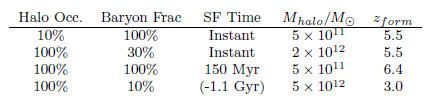
\includegraphics[scale=0.7]{Figuras/steindhart_table}
\caption{\label{fig:table1} Tabla 1 de \cite{steinhardt2016impossibly} con las variaciones descritas en el punto 5.}
\end{center}
\end{figure}

Encontramos que cada una de estas combinaciones requiere una física inverosímil, como que el 100\% de los bariones se conviertan en estrellas instantáneamente tras la virialización del halo o el 10\% de los bariones que forman estrellas sobre 1 Gyr antes de que el halo de materia oscura virialice, o contradiga otros resultados de observación. Por ejemplo, varias combinaciones requieren masas de halo por debajo de $10^{12}M_\odot$. Sin embargo, a $3.1 <z <4.7$, \cite{hildebrandt2009cars} utilizaron mediciones de agrupamiento en CFHTLS para encontrar que las galaxias a 25.5 mag se encuentran en halos de $\log M_{halo} / M_\odot = 12.3$. Una proporción similar produciría $\log M_{halo} / M_\odot = 12.8$ para galaxias masivas en $z = 6$. \cite{finkelstein2015increasing} utilizan observaciones de CANDELS para argumentar que la relación de materia oscura a barión disminuye hacia un redshift más alto, de modo que la relación de masa de halo a masa estelar es 50:1 en $z = 6$ y 40:1 en $z = 7$. Esto correspondería a $\log M_{halo} / M_\odot = 12.7$.\\

En resumen, las soluciones que dan una fracción de ocupación de halo plausible requieren una escala de tiempo inverosímil para la formación de estrellas, una fracción mucho más alta de bariones para convertirse en estrellas que el 10\% en los modelos actuales, o ambos. Cualquier solución con una relación estándar entre la masa de halo y la masa estelar de entre 50:1 y 100:1 ($M_{halo }= 5 \times 10^{12} - 10^{13} M_\odot$) requiere que la mayor parte de la formación estelar ocurra mucho antes del colapso inicial y la virialización. \textcolor{red}{Formación estelar extra halo}.

\subsection{Galaxias masivas en simulación de fusiones}
Se han realizado grandes esfuerzos para estudiar la formación de galaxias masivas y sus halos de materia oscura a través de simulaciones numéricas. La gran diferencia en los procesos físicos dominantes y de escala entre la fusión jerárquica y la formación de estrellas significa que las simulaciones no pueden investigar ambos procesos directamente, sino que usan recetas semianalíticas para conectar las propiedades de las galaxias masivas a sus halos.\\

Estas recetas intentan modelar la física bariónica en un nivel muy macroscópico y se basan en relaciones de redshift más bajas observadas entre las galaxias y sus halos anfitriones. Sin embargo, extrapolar estas relaciones a menudo conduce a resultados no físicos: la simulación Millennium  puede producir galaxias $M_\star = 10^{11}M_\odot$ en $z = 6$, pero viven en halos de materia oscura con $M = 10^{11.3}M_\odot$. Esta es una relación de masa de halo a masa estelar muy pequeña en varios frentes: en teoría, requeriría que los bariones se agrupen antes de gran parte de la materia oscura, así como casi todos los bariones que terminaron en estrellas por $z = 6$. Observacionalmente, estaría en conflicto con \cite{hildebrandt2009cars} y \cite{finkelstein2015increasing} relaciones de masa de halo a masa estelar discutidas en la sección anterior.\\

La simulación Illustris selecciona un conjunto de relaciones bariónicas que evitan estas extrapolaciones no físicas, lo que resulta en una función de masa estelar y una función de luminosidad similar a la función de masa de halo. Como resultado, las densidades numéricas simuladas de las galaxias masivas son consistentes con la observación a $M_\star 10^{10}M_\odot$ en $z\sim 4 - 6$, pero se producen muy pocas galaxias con $M_\star> 10^{10.5}M_\odot$, en desacuerdo con las densidades numéricas observadas en esa masa y redshift.\\

La conclusión de estas simulaciones es que existe un amplio consenso sobre la función de masa de halo, pero una libertad considerable para hacer coincidir esas masas de halo con las propiedades galácticas. Incluso dada esa libertad, las observaciones coincidentes requerirían que las masas estelares estén sobre-estimadas o que haya una desconexión aguda entre los bariones en las galaxias masivas y sus halos de materia oscura. Específicamente, las simulaciones son consistentes con las galaxias típicas en estos redshift, pero no pueden producir las galaxias más antiguas y masivas vistas en $z> 4$ con la introducción de una física razonable. Más bien, entonces, comprender estas galaxias parece requerir física adicional que aún no se incluye en estas simulaciones, ya sea física bariónica relacionada con la formación de estrellas o física de alta energía que altera el momento de la formación masiva de halo.

\section{Discusiones}
Hemos demostrado que las observaciones recientes de galaxias de alto redshift son inconsistentes con los modelos teóricos actuales de ensamblaje galáctico. Como principio general, cuando la teoría y la observación no están de acuerdo, históricamente es mejor creer el resultado de la observación. Sin embargo, en este caso las observaciones también se basan en supuestos teóricos no probados sobre la evolución estelar. Por lo tanto, algo está mal, pero ¿qué? Podemos dividir los posibles defectos y explicaciones en tres categorías posibles:
\begin{description}
\item[Fallo del ajuste o de la determinación del redshift:] Si las mediciones son incorrectas, lo más probable es que no esté en los redshift (ya que existen redshift espectroscópicos para muchas galaxias menos masivas en $z> 5$), sino más bien en el supuesto de que las plantillas derivadas de las galaxias con redshift más bajo pueden usarse en $z = 6$. Esto implica que la relación entre la masa de halo y la luminosidad monocromática cambia bruscamente por encima de $z = 4$. Como se discutió en el \cref{sec:ratio_halo_lum}, la explicación más probable para esta evolución sería una IMF claramente más pesada en los redshift más altos. Potencialmente, esto se puede probar en el futuro cercano utilizando tasas de supernova y, ciertamente, después del lanzamiento de JWST.\\

La espectroscopía posterior confirmó que las plantillas de redshift bajo arrojaron resultados correctos para cantidades inferidas como la masa estelar a $z <3$. Si esto se descompone en $z\sim 6$, significaría que los estudios puramente fotométricos ahora son insuficientes, ya que se deben desarrollar nuevos modelos y observacionalmente probado por JWST. Es inevitable que en algún momento los astrónomos se encuentren con este problema, pero sería desagradable descubrir que ocurre a un redshift más bajo de lo que se cree actualmente.

\item[Nueva Física de Agrupamiento:] Otra posibilidad es que los halos colapsen antes de lo permitido
según los modelos actuales, algo que resolvería simultáneamente el problema del quasar masivo de alto redshift también. Los tiempos de colapso actuales se derivan de la gravedad que actúa sobre perturbaciones que pueden confirmarse utilizando mediciones de fondo de microondas cósmicas, y por lo tanto, un colapso mucho más rápido de los halos requeriría la introducción de una nueva física de alta energía. Las posibles soluciones aquí podrían proporcionar nuevas y emocionantes restricciones sobre la naturaleza de la energía oscura o la materia oscura. Cabe señalar que muchos modelos de materia oscura que se consideran actualmente son WDM, que suprimiría la función de masa de halo $z\sim 6$ en lugar de mejorarla. La energía oscura con $w> -1$, podría mejorar la formación temprana de la estructura, aunque las observaciones de fondo cósmico de microondas crean una tensión considerable con el $w> -0.95$ requerido para resolver este problema.

\item[Formación estelar temprana:] Otra posibilidad es que los halos colapsen antes de lo permitido. Una solución bariónica está en lugar de permitir la formación de estrellas de la secuencia principal mucho antes que el colapso inicial de los halos. Dichas ideas tendrían que evadir las restricciones difíciles de ambas observaciones deredshift bajo, así como resolver el problema del enfriamiento para formar pequeñas estrellas con baja metalicidad. Además, observamos que si las estrellas iniciales se forman en pequeños grupos en lugar de en protogalaxias completamente formadas, el ``factor de agrupamiento'' en la reionización será mucho mayor de lo esperado, lo que resultará en una reionización mucho más rápida solo por la formación de estrellas de lo esperado actualmente. Si es así, esto será evidente en las mediciones de fluctuación de fondo infrarrojo.
\end{description}

Las tres respuestas tienen consecuencias importantes tanto para nuestra comprensión actual de las etapas iniciales de la formación galáctica como para nuestros planes futuros para estudiar galaxias de alto redshift. Por lo tanto, se necesitan mejores observaciones. Existe una esperanza considerable de que las observaciones de seguimiento ayuden a determinar si la primera de estas tres explicaciones es la correcta.

En lugar de especular sobre cuál es la mejor explicación, enfatizamos que los objetos de gran masa que salen de los estudios de alto redshift son ahora críticamente importantes. Los estudios futuros deberían concentrarse en encontrar y caracterizar estos objetos en cantidades suficientes para restringir cómo estas galaxias y sus halos co-evolucionan. Desde las primeras galaxias más masivas son raras, se necesitarán estudios de área amplios en la escala $> 1$ grado. Estos objetos ya no son simplemente un punto extra o dos en el último panel de una figura, sino que representan un problema clave en el corazón de la astronomía extragaláctica de alto redshift, y deben recibir la atención correspondiente.
\newpage
\bibliographystyle{plainnat}
\bibliography{references}

\newpage
\appendix
\section*{Planteamientos iniciales de cada día de trabajo}
Notas que pretenden estructurar el trabajo día a día
\subsection*{Agosto 2019}
A falta de terminar de analizar el paper de \cite{finkelstein2015increasing} y de hacer una lista de las dudas surgidas y propuestas a dar ya he leido el artículo de \cite{wang2019dominant} sobre las galaxias a redshift $z>3$ descubiertas por ALMA las cuales parecen ser abundantes y masivas y no detectables por el HST. Esto tumbaría la susposición de \cite{finkelstein2015increasing} de la no existencia o poca abundancia de las galaxías sub-milimétricas lo que modificaría la función de luminosidad y por tanto la relación de masa halo - masa estelar ya que en el paper de \cite{finkelstein2015increasing} se basa principalmente en ella. La propuesta de lo que quiero hacer hoy es lo siguiente:
\begin{enumerate}
\item Terminar el análisis de \cite{finkelstein2015increasing}. $\surd$
\item Como encaja las nuevas observaciones de \cite{wang2019dominant} en el paper de \cite{finkelstein2015increasing} $\surd$
\item Plantear como incluir los planteamientos de \cite{wang2019dominant}: 
\begin{enumerate}[i.]
\item Replantear la función de luminosidad de \cite{finkelstein2015increasing}.
\item Como encaja en el modelo jerárquico \citep{bower2006breaking}.
\item Las simulaciones de RAMSES nos pueden dar un orden distinto a la masa de los halos que encajen de una manera distinta de con la función de luminosidad. 
\end{enumerate}
\end{enumerate}

\subsection*{Septiembre 2019}
\subsubsection*{Semana 2: 9-15}
El artículo de \cite{wang2019dominant} parece indicar que algunas de las suposiciones en las que se basan los métodos de cálculo de las masa de halo están equivocados, por lo que el escenario más factible para la resolución del problema de \cite{steinhardt2016impossibly} sea el error observacional. Las tareas para esta semana son las siguientes:
\begin{enumerate}
\item Terminar el análisis de \cite{steinhardt2016impossibly}.
\item Leer el artículo de \cite{sheth2001ellipsoidal} y \cite{murray2013hmfcalc} que trata las estimaciones teóricas usadas para el cálculo de la función de masa de halo. Empezar con el resumen de \cite{sheth2001ellipsoidal}.
\item Terminar el punto 3 de agosto.
\item Escribir a Santi con los avances el domingo día 15 y plantear con él una reunión.
\end{enumerate}
\end{document}
